\documentclass{amsart}
%\documentclass[a4paper,10pt]{scrartcl}

\usepackage[utf8x]{inputenc}
\usepackage[british]{babel}
%\usepackage[a4paper, inner=0.5cm, outer=0.5cm, top=1cm,
%bottom=1.5cm, bindingoffset=1cm]{geometry}
\usepackage{amsmath}
\usepackage{amssymb, latexsym}
\usepackage{longtable}
\usepackage[table]{xcolor}
\usepackage{textcomp} 
\usepackage{graphicx}
\usepackage{enumitem}
\usepackage{hyperref}


\setlist[enumerate]{label*=\arabic*.}
\newtheorem{theorem}{Theorem}[section]
\newtheorem{example}{Example}[section]
\newtheorem{definition}{Definition}[section]
\newtheorem{proposition}{Proposition}[section]
\newtheorem{notation}{Notation}[section]


\title{EquivalentTo versus SubClassOf}
\author{Henriette Harmse}
\date{\today}

\pdfinfo{%
  /Title    (EquivalentTo versus SubClassOf)
  /Author   (Henriette Harmse)
  /Creator  ()
  /Producer ()
  /Subject  (DL)
  /Keywords ()
}

\begin{document}
  \maketitle
  
  In creating their first ontology, there are at least two aspects of \texttt{EquivalentTo} and \texttt{SubClassOf} that perplex users. The first is when to use \texttt{EquivalentTo} and when to use \texttt{SubClassOf}. The second problem is best illustrated by the following example:
  
  
\begin{small}
	\begin{verbatim} 
		ObjectProperty: a_to_b
		
		Class: A1
		   EquivalentTo: (a_to_b some B)
		
		Class: A2
		   SubClassOf: (a_to_b some B)
		
		Class: B
		
		Individual: b1
		   Types: 
		       B
		
		Individual: x
		   Facts:  
		       a_to_b  b1
	\end{verbatim}
\end{small}  


\begin{figure}
	%trim option's parameter order: left bottom right top
	\centering 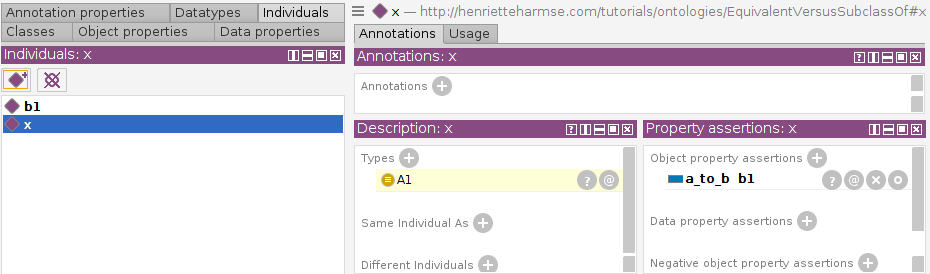
\includegraphics[trim = 0mm 0mm 0mm 0mm, clip, scale=0.4]{./images/xTypeOfA1.png}
	\caption{\texttt{x} is inferred to be of type \texttt{A1}}
\end{figure}
  
  When running a reasoner on this example, the individual \texttt{x} is inferred to be of type \texttt{A1}. What perplex users sometimes is that \texttt{x} is not inferred to be of type \texttt{A2} as well.
  
  
  \section{The difference between \texttt{EquivalentTo} and \texttt{SubClassOf}}
  The first thing to be aware of wrt \texttt{equivalentTo} is that 


\begin{small}
	\begin{verbatim} 
		Class: C
		   	EquivalentTo: D
	\end{verbatim}
\end{small}  

is an abbreviation for 

\begin{small}
	\begin{verbatim} 
		Class: C
		    SubClassOf: D
			
		Class: D
	        SubClassOf: C			
	\end{verbatim}
\end{small}   
  
The semantics of \texttt{SubClassOf} is subset. Thus, the above states that the set \texttt{C} is a subset of the set \texttt{D} and the set \texttt{D} is a subset of the set \texttt{C}. Which means that the sets \texttt{C} and \texttt{D} are exactly the same set. We say they are equivalent.

Note that if I know that the classes \texttt{C1} and \texttt{C2} are both subclasses of class \texttt{C}, there is nothing more I can say about how class \texttt{C1} relates to class \texttt{C2}. This is a bit like knowing that bicycles and trucks are both vehicles - I can say nothing more about how bicycles relate to trucks beyond knowing that they are both vehicles.


\section{Back to our initial example}
Understanding the semantics of \texttt{EquivalentTo} we can see that indeed the individual \texttt{x} is an instance of \texttt{A1}. Understanding the semantics of \texttt{SubClassOf} helps us to understand why \texttt{x} is not inferred to be of type \texttt{A2}. We know that \texttt{A2} is a subclass of \texttt{a\_to\_b some B} and that \texttt{x} is an instance of \texttt{a\_to\_b some B}, but there is nothing that can force the reasoner to infer that \texttt{x} is necessarily an instance of the class \texttt{A2}. This is illustrated in the next figure.

\begin{figure}
	%trim option's parameter order: left bottom right top
	\centering 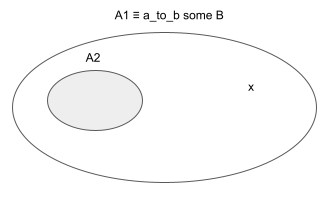
\includegraphics[trim = 0mm 0mm 0mm 0mm, clip, scale=0.9]{./images/EquivalenceVersusSubClassOf-Cropped.png}
	\caption{\texttt{A2} and \texttt{x} wrt \texttt{a\_to\_b some B}}
\end{figure}


\section{When to use \texttt{EquivalentTo} versus \texttt{SubClassOf}}
\texttt{EquivalentTo} is used for definitions. That is when you want to state the necessary and sufficient conditions for a concept.

\texttt{SubClassOf} is used when you want to define a hierarchy from the most general to the most specific. I.e., it is typically what you see in taxonomies or in object oriented programming languages where one can define class hierarchies.

\section{Conclusion}
In this post I explained the difference between \texttt{EquivalentTo} versus \texttt{SubClassOf} and how they are used, as well as some inferences that
may be confusing to new users. You can find the example ontology on \href{https://github.com/henrietteharmse/henrietteharmse/tree/master/blog/tutorial/ontologies/examples}{github}
  
  \bibliographystyle{amsplain}
  \bibliography{../../../BibliographicDetails_v.0.1}
 
\end{document}
